\let\negmedspace\undefined
\let\negthickspace\undefined
\documentclass[journal]{IEEEtran}
\usepackage[a5paper, margin=10mm, onecolumn]{geometry}
%\usepackage{lmodern} % Ensure lmodern is loaded for pdflatex
\usepackage{tfrupee} % Include tfrupee package

\setlength{\headheight}{1cm} % Set the height of the header box
\setlength{\headsep}{0mm}     % Set the distance between the header box and the top of the text

\usepackage{gvv-book}
\usepackage{gvv}
\usepackage{cite}
\usepackage{amsmath,amssymb,amsfonts,amsthm}
\usepackage{algorithmic}
\usepackage{graphicx}
\usepackage{textcomp}
\usepackage{xcolor}
\usepackage{txfonts}
\usepackage{listings}
\usepackage{enumitem}
\usepackage{mathtools}
\usepackage{gensymb}
\usepackage{comment}
\usepackage[breaklinks=true]{hyperref}
\usepackage{tkz-euclide} 
\usepackage{listings}
% \usepackage{gvv}                                        
\def\inputGnumericTable{}                                 
\usepackage[latin1]{inputenc}                                
\usepackage{color}                                            
\usepackage{array}                                            
\usepackage{longtable}                                       
\usepackage{calc}                                             
\usepackage{multirow}                                         
\usepackage{hhline}                                           
\usepackage{ifthen}                                           
\usepackage{lscape}
\begin{document}

\bibliographystyle{IEEEtran}
\vspace{3cm}

\title{1.8.12}
\author{EE24BTECH11001 - Aditya Tripathy
}
 \maketitle
% \newpage
% \bigskip
{\let\newpage\relax\maketitle}

\renewcommand{\thefigure}{\theenumi}
\renewcommand{\thetable}{\theenumi}
\setlength{\intextsep}{10pt} % Space between text and floats


\numberwithin{equation}{enumi}
\numberwithin{figure}{enumi}
\renewcommand{\thetable}{\theenumi}


\textbf{Question}:\\
Find the point on $X$ axis which is equidistant from \myvec{7\\6} and \myvec{3\\4}.
\\
\textbf{Solution: }\\
Let the desired point on the $X$ axis be C $\myvec{x \\ 0}$. Let $A$ and $B$ be the above points respectively.
Let $S$ be any point on the perpendicular bisector of $AB$
\begin{align} 
    ||A-S|| = ||B-S||\\
    \implies \sqrt{\brak{A-S}^\top \brak{A-S}} =  \sqrt{\brak{B-S}^\top \brak{B-S}} \\
    \implies  \brak{A-S}^\top \brak{A-S} = \brak{B-S}^\top \brak{B-S} \\
    ||A||^2 - S^\top A - A^\top S + ||S||^2 =  ||B||^2 - S^\top B - B^\top S + ||S||^2 \\
    \implies 2B^\top S - 2A^\top S = ||B||^2 - ||A||^2\\
    \implies 2\brak{B-A}^\top S = ||B||^2 - ||A||^2 \\
\end{align}
Now we have the line representing perpendicular bisector of line joining $A$and $B$.
The solution $S$ is found by solving the previous eqution with the eqution for $X$ axis.
\begin{align}
    m^\top S = 0\\
\end{align}
where m = \myvec{0 \\ 1}.\\
So, the matrix equation to solve becomes,
\begin{align}
    \myvec{B-A &  m}^\top S = \myvec{\frac{||B||^2 - ||A||^2}{2}\\ 0}
\end{align}

On solving,
\begin{align}
    \myvec{-4 & -2 \\0 & 1}S = \myvec{-30 \\ 0}\\
    \myvec{-4 & -2 & -30 \\ 0 & 1 & 0} \xrightarrow{R_1 = 2R_2 + R_1 } \myvec{-4 & 0 & -30 \\ 0 & 1 & 0}\\
    \myvec{-4 & 0 & -30 \\ 0 & 1 & 0} \xrightarrow{R_1 = \frac{R_1}{-4}}
    \myvec{1 & 0 & 7.5 \\ 0 & 1 & 0}\\
    \implies C = \myvec{7.5\\0}\\
\end{align}
Therefore \myvec{7.5\\0} is the required point on $X$-axis.    
\begin{figure}[h!]
   \centering
   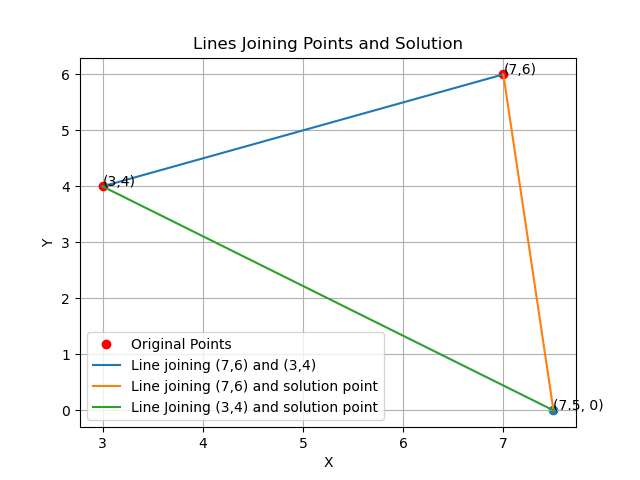
\includegraphics[width=0.7\linewidth]{figs/fig.png}
   \caption{Line joining the three given points}
\end{figure}
\end{document}  
